\section{Sewer interconnection}\label{se:sewer_interconnection}
This section will explain how interconnection between channels are modeled and how the mixing between wastewater and wastewater with chemicals.

In figure \ref{fig:interconnections} an illustration of a interconnection between two flows are shown.

\begin{figure}[H]
\centering
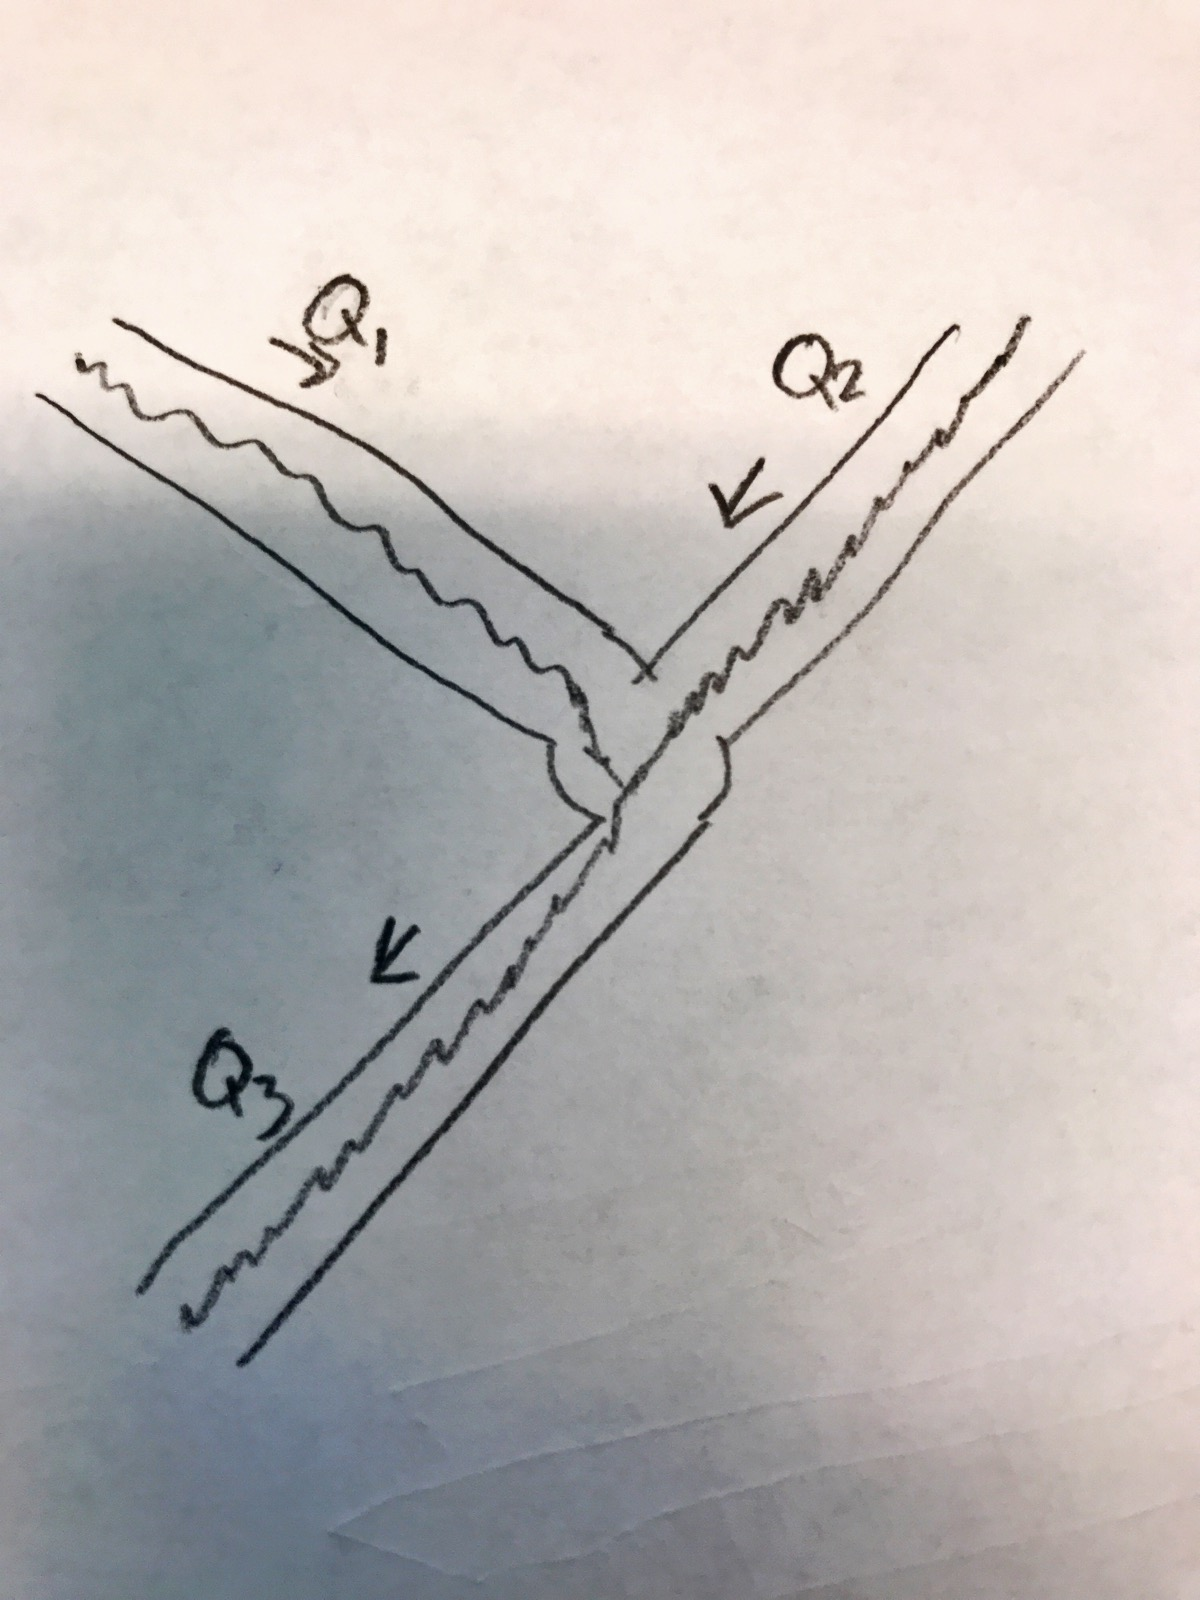
\includegraphics[width=0.30\textwidth]{report/modeling/pictures/interconnections.jpg}
\caption{Illustration of an interconnection between two flow inputs and one output.}
\label{fig:interconnections}
\end{figure} \fxnote{Ny tegning}

The two channels $Q_1$ and $Q_2$ are connected at the end of each channel here the wastewater from the two channels will be added up. The flow $Q_3$ is calculated as:

\begin{equation}
	Q_3 = Q_1 + Q_2 	
\end{equation} 

For the mixing between two flows where one of them is transporting chemicals will be done in similar way as for flows. 

\begin{equation}
	C_3 = \frac{C_1 Q_1 + C_2 Q_2}{Q_3}
\end{equation}

This is done to keep the same amount of chemicals within the wastewater, as the algorithm for transporting chemicals is depended on flow, as seen in section \ref{se:transport_of_concentrate}. If it is not calculated like this, thus when the flow is increasing the same will the chemicals within the wastewater, hence it is needed to divided by $Q_3$ to get the right amount of chemicals in the wastewater.  